\begin{table}[h]
	\centering
	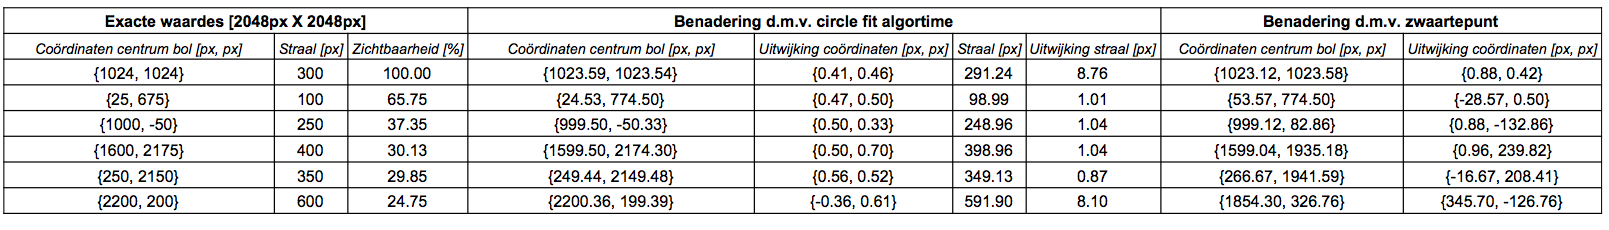
\includegraphics[width=1\textwidth]{TestData.png}
	\caption{Deze testdata van de \textit{ImageCalculation} geeft de verschillen weer tussen beide algoritmes die gebruikt worden om de afstand van de bol te berekenen. Het is duidelijk dat het circle-fitalgoritme beduidend minder afwijkt van de correcte waardes dan het algoritme op basis van het zwaartepunt. Hoe minder de bol procentueel zichtbaar is, hoe groter de afwijking. Ook wordt de berekende straal en afwijkingen weergegeven. Dit is enkel mogelijk bij het circle-fitalgoritme. }
\end{table}